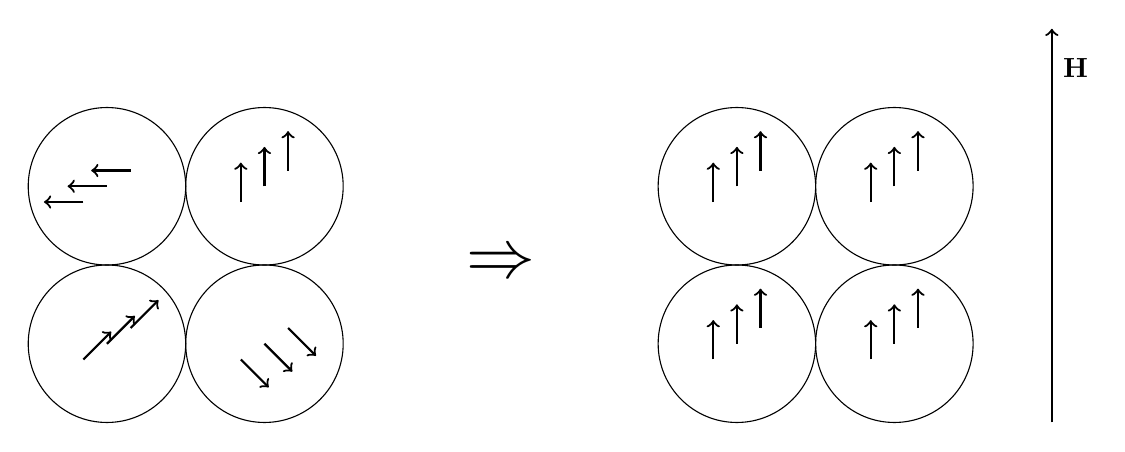
\begin{tikzpicture}[scale=1]

% --- Primo gruppo (sinistra) ---
\foreach \x/\y/\angle in {0/0/45, 2/0/-45, 0/2/180, 2/2/90} {
    \draw[rounded corners] (\x,\y) circle [x radius=1cm, y radius=1cm];
    % Più frecce parallele con variazione verticale e più corte
    \foreach \dx/\dy in {-0.3/-0.2, 0/0, 0.3/0.2} {
        \draw[->, thick] (\x+\dx,\y+\dy) -- ++({0.5*cos(\angle)},{0.5*sin(\angle)});
    }
}

% Freccia centrale
\node at (5,1) {\Huge $\Rightarrow$};

% --- Secondo gruppo (destra) ---
\foreach \x/\y in {8/0, 10/0, 8/2, 10/2} {
    \draw[rounded corners] (\x,\y) circle [x radius=1cm, y radius=1cm];
    % Più frecce parallele verso l'alto con variazione verticale e più corte
    \foreach \dx/\dy in {-0.3/-0.2, 0/0, 0.3/0.2} {
        \draw[->, thick] (\x+\dx,\y+\dy) -- ++(0,0.5);
    }
}

% Freccia H
\draw[->, thick] (12,-1) -- (12,4);
\node at (12.3,3.5) {\textbf{H}};

\end{tikzpicture}